\documentclass[aoas,preprint]{imsart}
%\RequirePackage{mdframed}
%\usepackage{mdframed}
\usepackage[framemethod=TikZ]{mdframed}
\RequirePackage[OT1]{fontenc}
\usepackage[utf8x]{inputenc}
\RequirePackage{amsthm,amsmath}
\RequirePackage{natbib}
\RequirePackage[colorlinks,citecolor=blue,urlcolor=blue]{hyperref}

\usepackage[sc]{mathpazo}
\usepackage{amsmath, wrapfig}
\usepackage{dsfont}
\usepackage{graphicx}
\usepackage{caption}
\DeclareCaptionFormat{myformat}{\hrulefill \\ #1#2#3}
\DeclareCaptionFont{small}{\footnotesize}
\DeclareCaptionFont{blue}{\color{blue}} 
\DeclareCaptionFont{bf}{\bfseries}
\captionsetup[figure]{format=myformat,labelfont={blue,bf,small},font=small}
\usepackage{booktabs}% http://ctan.org/pkg/booktabs

%\usepackage{algorithm,algcompatible,amsmath}
\usepackage{algorithm, eqparbox,array}% http://ctan.org/pkg/algorithms
\usepackage{algpseudocode}% http://ctan.org/pkg/algorithmicx
%\usepackage{xcolor}
%\usepackage[usenames, dvipsnames]{color}
\usepackage{color}
\RequirePackage{xcolor}
%\usepackage{mdframed}





 \setlength{\parskip}{1ex}
\newtheorem{lemma}{Lemma}
\newtheorem{theorem}{Theorem}
\newtheorem{prop}{Proposition}
\DeclareGraphicsRule{.tif}{png}{.png}{`convert #1 `dirname #1`/`basename #1 .tif`.png}

\begin{document}

Supplementary Material 

main document

{A compositional model to assess expression changes from single-cell RNA-seq data}

by Ma, Korthauer, Kendziorski, and Newton



Contents
\begin{enumerate}
\item Synthetic Data
\item Data sets 
\item \verb+EBseq+
\item \verb+modalclust+
\item choosing $K$ by validity score
\item Randomized k-means
\item Proofs: 
\end{enumerate}

\noindent
{\bf Synthetic Data}

\begin{figure}[h!]
  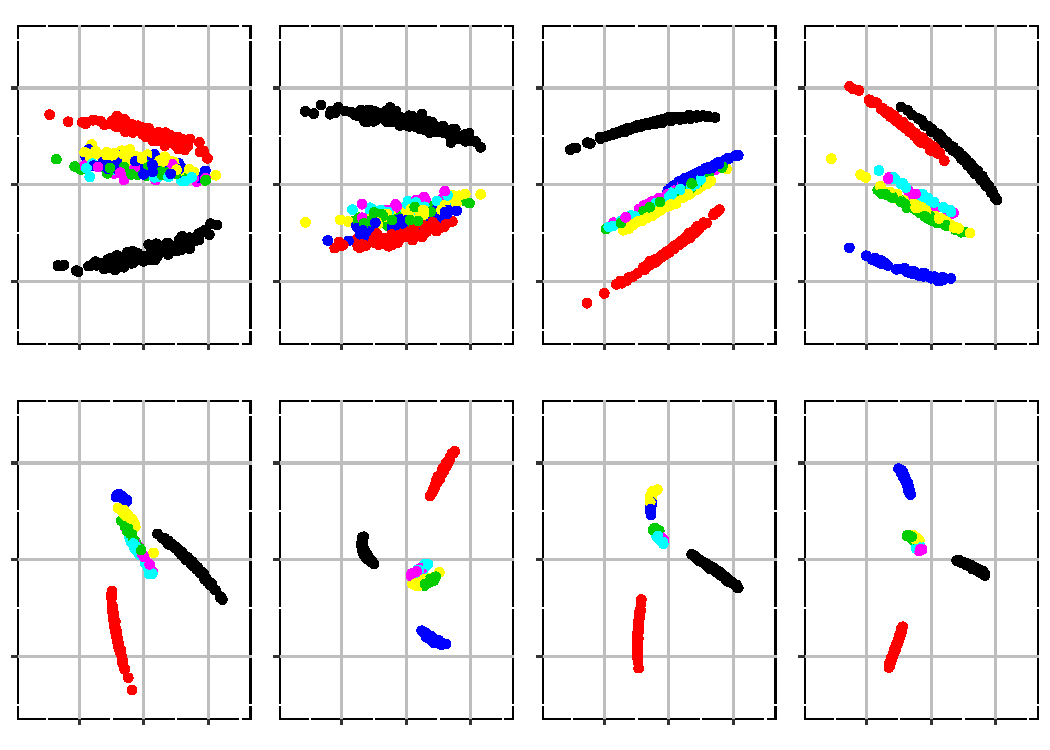
\includegraphics[ width = 0.8\textwidth]{Figs/pca.pdf}
  \caption{first two principal components of transcripts under different parameters for simulated data. Different parameters resulted in different degree of separation of subtypes. We have 4 different settings for hyper-parameters of simulation, each setting has 2 replicates}
  \label{fig:4}
\end{figure}




\noindent
{\bf Data sets}


\begin{table}[ht]
\small
\centering
\begin{tabular}{ |p{2cm}|p{5cm}|p{2cm}|p{2cm}|p{2cm}|p{1cm}|}
\hline
 Data set & Conditions & Number of cells/condition & Organism  & Ref & K\\ \hline \hline
GSE52529 & T0 vs T24 & 96,96 & human & \citep{Trapnell} & 6\\ \hline
GSE57872 & patient1 vs patient2 & 192,96 & human & \citep{Patel} & 7 \\ \hline
GSE48968-GPL13112 & BMDC (2h LPS stimulation) vs 6h LPS & 96,96 & mouse & \citep{Shalek} & 8\\ \hline
GSE60749-GPL13112 & serum + LIF vs  2i + LIF & 90,94 & mouse & \citep{Kumar} & 3\\ \hline
GSE74596 & NKT1 vs NTK2 & 46,68 & mouse & \citep{Engel} & 5\\ \hline
EMTAB2805 & G1 vs G2M & 95,96 & mouse & \citep{EMTAB} & 7\\ \hline
GSE71585-GPL13112 &Gad2tdTpositive vs Cux2tdTnegative  & 80,140 & mouse & \citep{Tasic} & 7\\ \hline
GSE64016 & G1 vs G2 & 91,76 & human & \citep{oscope} & 8 \\ \hline
GSE79102 & patient1 vs patient2 & 51, 89 & human & \cite{sc3} & 4\\ \hline
GSE45719 & 16-cell stage blastomere vs mid blastocyst cell & 50, 60 & mouse & \citep{Deng193} & 5\\ \hline
GSE63818 & Primordial Germ Cells, develop- mental stage: 7 week gestation vs Somatic Cells, developmental stage: 7 week gestation & 40,26 & mouse & \citep{Guo} & 6\\ \hline
GSE75748 & DEC vs EC & 64, 64 & human & \citep{chu} & 9\\ \hline
GSE84465 & neoplastic cells vs non-neoplastic cells & 546, 664 & human & \citep{Darmanis} & 9\\ \hline
\end{tabular}
\captionof{table}{datasets used for comparisons of DD analysis under different methods}
\end{table}




%\begin{figure}[H]
%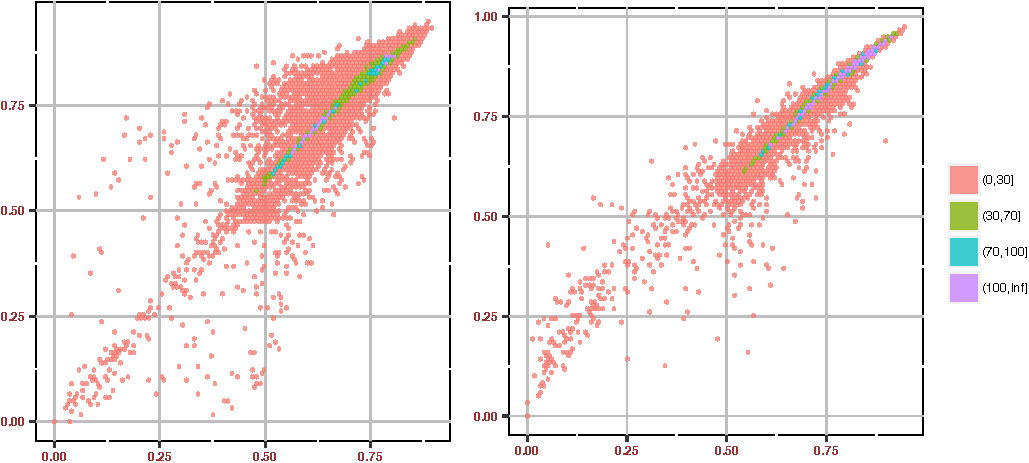
\includegraphics[width = 0.6\textwidth]{Figs/sim.pdf}
% \caption{ comparison of posterior probabilities of being DD among different number of subtypes, when we underestimate the number of subtypes, the difference is huge, see PDD between 6 subtypes and 7 subtypes. There is an approximate horizontal line with massive points at the top of left panel, which indicate that we underestimate lots of DD genes due to underestimate the number of subtypes. While in the case when we overestimate the number of subtypes 7 subtypes vs. 8 subtypes, though inflating PDD but the variation of difference is small, from 6 to 8 subtypes the PDD become more linear related.}
%  \label{fig:6}
%\end{figure}




\begin{figure}[h]
\vspace{-\parskip}
\minipage{0.5\textwidth}
  \includegraphics[width=\textwidth]{Figs/sim_67.png}
\endminipage\hfill
\minipage{0.5\textwidth}
  \includegraphics[width=\textwidth]{Figs/sim_78.png}
  \endminipage
\caption{comparison of posterior probabilities of being DD among different number of subtypes, when we underestimate the number of subtypes, the difference is huge, see PDD between 6 subtypes and 7 subtypes. There is an approximate horizontal line with massive points at the top of left panel, which indicate that we underestimate lots of DD genes due to underestimate the number of subtypes. While in the case when we overestimate the number of subtypes 7 subtypes vs. 8 subtypes, though inflating PDD but the variation of difference is small, from 6 to 8 subtypes the PDD become more linear related.}
\end{figure}





\noindent
{\bf EBSeq}

Suppose we have $K$ subtypes, let $X_g^I = X_{g, 1}^I, ... , X_{g, S_1}^I$ denote transcripts at gene $g$ from subtype $I, I = 1, ... K$.  In the EBSeq model it assumed that counts within subtype $I$ are distributed as Negative Binomial:
$X_{g, s}^I | r_{g,s}, q_g^I \sim NB(r_{g,s}, q_g^I)$ Where

\begin{eqnarray*}
P(X_{g,s}^I | r_{g,s}, q_g^I ) = {X_{g,s} + r_{g,s} - 1 \choose X_{g,s} }(1 - q_g^I)^{X_{g,s}^I} (q_g^I)^{r_{g,s}}
\end{eqnarray*}
and $\mu_{g,s}^I = r_{g,s}(1 - q_g^I) / q_g^I; \sigma_{g,s}^I = r_{g,s}(1 - q_g^I)/ (q_g^I)^2.$

The EBSeq model assumed a prior distribution on $q_g^I : q_g^I | \alpha, \beta^{I_g} \sim Beta(\alpha, \beta^{I_g}).$ The hyperparameter $\alpha$ is shared by all the isoforms and $\beta^{I_g}$ is $I_g$ specific. We further assume that $r_{g,s} = r_{g,0}*l_s$ where $r_{g,0}$ is an isoform specific parameter common across subtypes and $r_{g,s}$ depends on it through the sample-specific normalization factor $l_s$ 

What we are interested at those $K$ groups comparison is the expression pattern, through EBSeq modeling we are able to obtain posterior probabilities over 

\begin{eqnarray*}
M_{g,\pi} = \{ \theta \in \Theta: \; \mu_{g,k} = \mu_{g,k'} \iff k,k' \in b, b \in \pi \}.
\end{eqnarray*}

For any partition $\pi$ of $K$ elements. 

For example $K = 3$, there are 5 expression pattern, $P_1, P_2, ..., P_5$ 

\begin{align*}
&P1: q_g^1 = q_g^2 = q_g^3\\
&P2: q_g^1 = q_g^2 \neq q_g^3\\
&P3: q_g^1 \neq q_g^2 = q_g^3\\
&P4: q_g^1 = q_g^3 \neq q_g^2\\
&P5: q_g^1 \neq q_g^2 \neq q_g^3 \text{ and } q_g^1 \neq q_g^3
\end{align*}

Under the assumption that two groups $I$ and $J$ share the same $q_g$ we can pool the counts from the two groups by viewing them come from same distribution i.e. $X_g^{I, J} | r_{g,s}, q_g \sim NB(r_{g,s}, q_g)$, $q_g | \alpha, \beta^{I_g} \sim Beta(\alpha, \beta^{I_g})$ and obtained the prior predictive function $f_0^{I_g}(X_g^{I,J}) = \int_0 ^1 P(X_g^{I,J} | r_{g,s}, q_g) * P(q_g | \alpha, \beta^{I_g}) dq_g = \Big[ \overset{S}{\underset{s = 1}{\prod}} {X_{g,s} + r_{g,s} - 1 \choose X_{g,s}} \Big] \frac{Beta(\alpha + \Sigma_{s = 1}^S r_{g,s}, \beta^{I_g} + \Sigma_{s = 1}^S X_{g,s})}{Beta(\alpha, \beta^{I_g})}$.  Consequently, we have prior predictive function for $P1, ..., P5$ as

\begin{align*}
&g_1^{I_g}(X_g^{1,2,3}) = f_0^{I_g}(X_g^{1,2,3})\\
&g_2^{I_g}(X_g^{1,2,3}) = f_0^{I_g}(X_g^{1,2})f_0^{I_g}(X_g^3)\\
&g_3^{I_g}(X_g^{1,2,3}) = f_0^{I_g}(X_g^1)f_0^{I_g}(X_g^{2,3})\\
&g_4^{I_g}(X_g^{1,2,3}) = f_0^{I_g}(X_g^{1,3})f_0^{I_g}(X_g^2)\\
&g_5^{I_g}(X_g^{1,2,3}) = f_0^{I_g}(X_g^1)f_0^{I_g}(X_g^2)f_0^{I_g}(X_g^3)\\
\end{align*}

Then the marginal distribution of counts $X_g^{1,2,3}$ is $\overset{5}{\underset{k = 1}{\Sigma}} p_k g_k^{I_g}(X_g^{1,2,3})$, where proportion parameters $p_k$ satisfying $\overset{5}{\underset{k = 1}{\Sigma}} p_k = 1$ and are estimated by EM algorithm. Thus, the posterior probability of an expression pattern $k$ is obtained by:
\begin{eqnarray*}
\frac{p_k g_k(X_g^{1,2,3})}{\overset{5}{\underset{k = 1}{\Sigma}} p_k g_k^{I_g}(X_g^{1,2,3})}
\end{eqnarray*}


\noindent 
{\bf modalclust}


{Product Partition Model}
Let $X = (X_1, X_2, ...,X_n)$ be $n$ one dimension observed data, given a partition for the data $\pi = \{S_1, ..., S_q\}$, where $S_i$ are disjoint subsets of $\{1,2,...,n\}$ and $\bigcup_{i = 1}^{q} S_i = \{1,2,...,n\}$. The likelihood for $X$ satisfying such partition is 
\begin{eqnarray*}
p(X|\pi) = \overset{q}{\underset{i = 1}{\prod}}f(X_{S_i})
\end{eqnarray*}

where $X_{S_i}$ is the vector of observations corresponding to the items of component $S_i$, The component likelihood $f(X_{S})$ is defined for any non-empty component $S$ and can take any form. The partition $\pi$ is the only parameter we are interested at. 
Any other parameters that may have been involved in the model have been integrated over their prior.

The prior distribution for a partition $\pi$ is also taken as a product form. We use the partition that maximize the posterior $p(\pi | X) \propto p(X|\pi) p(\pi)$ as the estimated clustering of $X$.

Dahl demonstrated by some choice of $f$ and prior of $\pi$, we can reduce the time complexity of finding the MAP partition from factorial($n$) to $O(n^2)$ \cite{ref:dahl},  
And the crucial condition for $f$ is that if $X_{S_1}$ and $X_{S_2}$ are overlapped in the sense that  min$\{X_{S_2}\}  <$ max$\{X_{S_1}\}  <$ max$\{X_{S_2}\}$ or min$\{X_{S_1}\}  <$ max$\{X_{S_2}\}  <$ max$\{X_{S_1}\}$, $X_{S_1^*} and X_{S_2^*}$ be the sets of swapping one pair of those overlapped terms and keep the other unchanged. Then $f(X_{S_1}) f(X_{S_2}) \leq f(X_{S_1^*}) f(X_{S_2^*})$. Under such condition, we know that possible MAP candidates must be those partition that for any two subgroups of data, all the data from subgroup1 has to be either greater or smaller than all the data from subgroup2.


In Poisson-Gamma Model we assuming:

\begin{align*}
X_i | \pi, \lambda &\sim Poisson(X_i | \lambda_1\textbf{I}\{i\in S_1\} + ... + \lambda_q\textbf{I}\{i \in S_q\})\\
\pi &\sim p(\pi)\\
\lambda_j &\sim Gamma(\alpha_0, \beta_0)
\end{align*}

where $p(\pi)\propto \overset{q}{\underset{i = 1}{\prod}}\eta_0\Gamma(|S_i|)$. Integrate out $\lambda$, $f(X_{S})$ is obtained as:

\begin{eqnarray*}
f(X_{S}) = \frac{\beta^\alpha}{(|S| + \beta)^{\underset{i \in S}{\Sigma} X_i + \alpha}} \frac{\Gamma(\underset{i \in S}{\Sigma} X_i  + \alpha)}{\Gamma(\alpha)} \frac{1}{\underset{i \in S}{\prod }X_i}
\end{eqnarray*}

$f(X_S)$ still satisfying the condition mentioned

\begin{proof}
if $X_{S_1}$ and $X_{S_2}$ are overlapped, without loss of generality, we assume min$\{X_{S_2}\}  <$ max$\{X_{S_1}\}  <$ max$\{X_{S_2}\}$, and we swap max$\{X_{S_1}\}$ with min$\{X_{S_2}\}$ and keep the rest unchanged or we could also swap max$\{X_{S_1}\}$ with max$\{X_{S_2}\}$. We denote the new set forming by swap of max$\{X_{S_1}\}$ with min$\{X_{S_2}\}$  as $S_1^*$ and $S_2^*$ and swap of max$\{X_{S_1}\}$ with max$\{X_{S_2}\}$ as $S_1^{**}, S_2^{**}$ accordingly. 

Then we need to show  at least one of the following happens 
\begin{align}
&f(X_{S_1^*}) f(X_{S_2^*}) \geq f(X_{S_1}) f(X_{S_2})\\
&f(X_{S_1^{**}}) f(X_{S_2^{**}}) \geq f(X_{S_1}) f(X_{S_2})
\end{align}


Let $a =$ max$\{X_{S_1}\}$, $b = $ min$\{X_{S_2}\}$ and $c = $ max$\{X_{S_2}\}$. $h_1 = \underset{i \in S_1}{\Sigma} X_i - a$ and $h_2 = \underset{i \in S_2}{\Sigma} X_i - b$, $n_1$ and $n_2$ are the number of elements in $S_1$ and $S_2$. Then 
\begin{align*}
f(X_{S_1^*}) f(X_{S_2^*}) &\geq f(X_{S_1}) f(X_{S_2})\\
&\iff\\
\frac{\Gamma(h_1 + a + \alpha)}{(n_1 + \beta)^{h_1 + a +\alpha}} \frac{\Gamma(h_2 + b + \alpha)}{(n_2 + \beta)^{h_2 + b + \alpha}} &\leq \frac{\Gamma(h_2 + a + \alpha)}{(n_2 + \beta)^{h_2+ a +\alpha}} \frac{\Gamma(h_1 + b + \alpha)}{(n_2 + \beta)^{h_1 + b + \alpha}}\\
&\iff\\
\frac{\Gamma(h_1 + a + \alpha)}{\Gamma(h_1 + b + \alpha)} \frac{\Gamma(h_2 + b + \alpha)}{\Gamma(h_2 + a + \alpha)} &\leq (\frac{n_1 + \beta}{n_2 + \beta})^{a - b} \\
\end{align*}

Left hand side of above formula is $\text{LHS}_1 = \frac{(h_1 + b + \alpha)...(h_1 + a - 1 + \alpha)}{(h_2 + b + \alpha) ... (h_2 + a - 1 + \alpha)}$ by the property of Gamma function and $X_i$ are integer.

Similarly,
\begin{align*}
f(X_{S_1^{**}}) f(X_{S_2^{**}}) &\geq f(X_{S_1}) f(X_{S_2})\\
&\iff\\
\frac{\Gamma(h_2 + c + \alpha)}{\Gamma(h_2 + a + \alpha)} \frac{\Gamma(h_1 + a + \alpha)}{\Gamma(h_1 + c + \alpha)} &\leq (\frac{n_2 + \beta}{n_1 + \beta})^{c - a} \\
\end{align*}

 Left hand side of above formula is $\text{LHS}_2 = \frac{(h_2 + a + \alpha)...(h_2 + c - 1 + \alpha)}{(h_1 + a + \alpha) ... (h_1 + c - 1 + \alpha)}$
 
If $h_1 \leq h_2$, then $\text{LHS}_1 \leq (\frac{h_1 + a - 1 + \alpha}{h_2 + a  - 1 + \alpha})^{a - b}$ and $\text{LHS}_2 \leq (\frac{h_2 + c - 1 + \alpha}{h_1 + c  - 1 + \alpha})^{a - b}$

So if $\frac{h_1 + a - 1 + \alpha}{h_2 + a  - 1 + \alpha} \leq \frac{n_1 + \beta}{n_2 + \beta} $ then (12) holds, if $\frac{h_2 + c - 1 + \alpha}{h_1 + c  - 1 + \alpha} \leq \frac{n_1 + \beta}{n_2 + \beta}$ then (13) holds

We multiply those two inequalities, we found that $\frac{h_1 + a - 1 + \alpha}{h_2 + a  - 1 + \alpha} * \frac{h_2 + c - 1 + \alpha}{h_1 + c  - 1 + \alpha} = \frac{h_1 + a - 1 + \alpha}{h_1 + c  - 1 + \alpha} * \frac{h_2 + c - 1 + \alpha}{h_2 + a  - 1 + \alpha} \leq 1$ as $c > a$ and $h_1 \leq h_2$ But $\frac{n_1 + \beta}{n_2 + \beta} * \frac{n_1 + \beta}{n_2 + \beta} = 1$. At least one equality holds, consequently at least one of (12) and (13) holds.

Similar proof for the case $h_1 > h_2$. 





\end{proof}


\noindent
{\bf Choosing $K$ by validity score:}

In order to determine the number of clusters, we consider the change of {\em validity} = $\frac{\textbf{intra}}{\textbf{inter}}$ defined in \cite{selK}, where $\textbf{intra} = \frac{1}{N}\overset{K}{\underset{i = 1}{\Sigma}}\underset{x \in C_i}{\Sigma} ||x - z_i||^2$, $\textbf{inter} = mean( || z_i - z_j||^2), i = 1,2,...,K-1. j = i+1,...,K$ and $z_i$ is the center(medoids) of cluster $i$. $\textbf{intra}$ is the average of distance of a point to its corresponding cluster center, which measures the compactness of clusters. We made a small change here, in original paper $\textbf{inter}$ was defined as minimum distance between medoids, we use average instead for the purpose of getting a smoother quantity. $\textbf{inter}$ is the average distance of two cluster centers, which measures the separation between clusters. We want to have a small intra-cluster distance and a big inter-cluster distance, consequently we wnat to minimize the {\em validity}. From empirical study, we constantly observe a monotone decreasing relation between number of clusters and {\em validity}. However this quantity stabilize when $K$ is sufficiently large. The stopping rule for searching $K$ is when $|validity_{K} - min(validity_K) | < \epsilon$ is satisfied.





\noindent
{\bf Randomized k-means}
\subsection{simulation}
We random generate one-dimensional data $X$ from a mixture of 5 normal distributions with different means and same variance. We compare clustering results between random weighting and bayesian clustering with Dirichlet process as prior in terms of posterior probabilities that two elements belong to the same class given the whole data and adjusted rand index comparing to the underlying true class label (Fig 12). 

\begin{figure}[h]
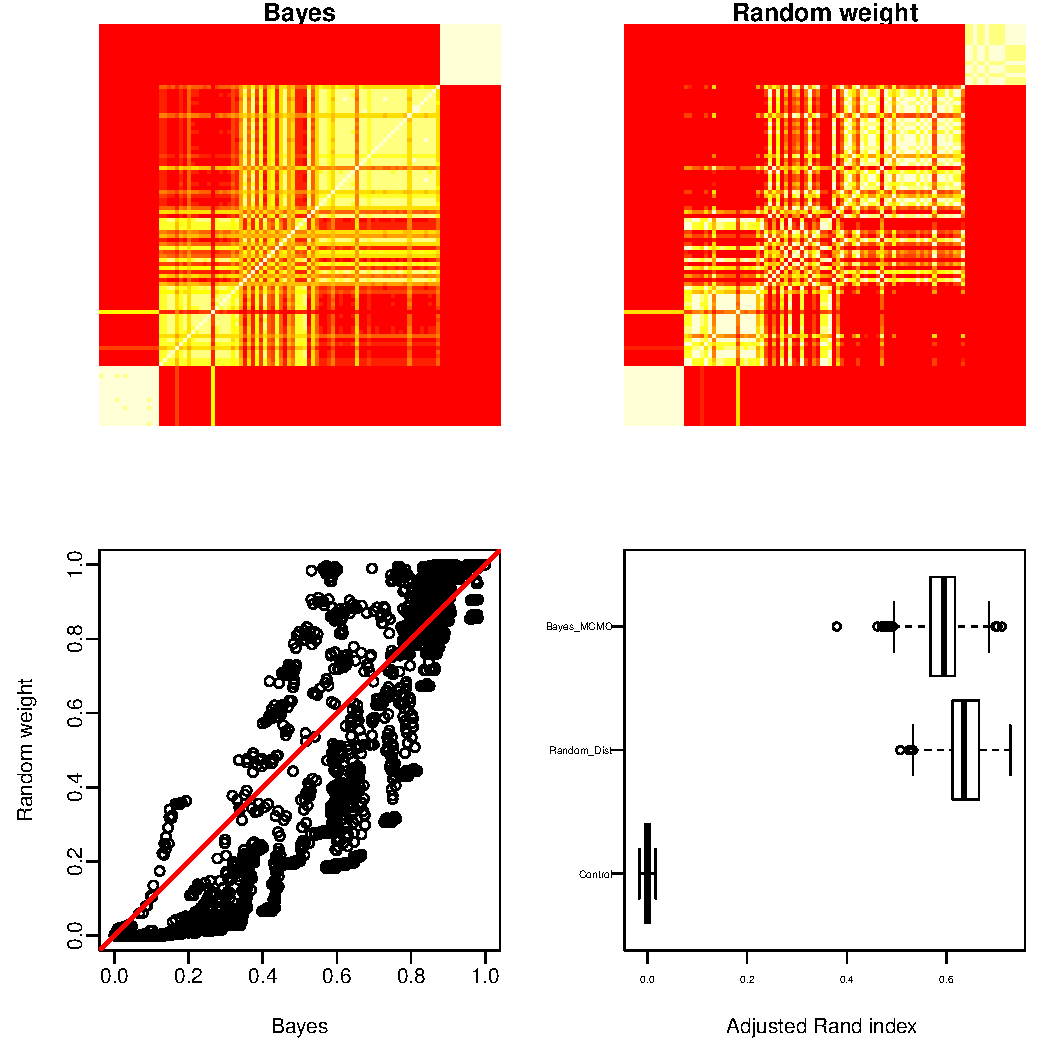
\includegraphics[scale = 1]{Figs/try7-g.pdf}
 \caption{comparison between random weighting scheme and bayesian clustering procedure in terms of posterior probabilities that two elements belong to the same class given the whole data and adjusted rand index comparing to the underlying true class label}
  \label{fig:1}
\end{figure}

\subsection{empirical study}




\noindent
{\bf Double Dirichlet Model:}

On the double Dirichlet masses, using notation as in Section 2.3 we have density functions:


\begin{eqnarray*}
p_\pi(\phi,\psi) =
         q_\pi( \Phi_\pi, \Psi_\pi  ) \, \prod_{b \in \pi}  \left[
         p( \tilde \phi_b ) p( \tilde \psi_b ) \right]
\end{eqnarray*}
with
\begin{eqnarray*}
q_\pi( \Phi_\pi, \Psi_\pi  )
= \frac{\Gamma(\sum_{b\in \pi} \beta_b)}{
 \prod_{b \in \pi} \Gamma( \beta_b )} \left[\prod_{b \in \pi} \Phi_b^{\beta_b-1} \right] \,
 1\left[ \Phi_\pi = \Psi_\pi \right]
\end{eqnarray*}
and
\begin{eqnarray*}
p( \tilde \phi_b ) =
\frac{ \Gamma( \sum_{k\in b} \alpha_k ) }{ \prod_{k\in b} \Gamma(\alpha_k) }
 \prod_{k \in b} \tilde \phi_k^{\alpha_k -1 },
\qquad
p( \tilde \psi_b )
=
\frac{ \Gamma( \sum_{k\in b} \alpha_k ) }{ \prod_{k\in b} \Gamma(\alpha_k) }
\prod_{k \in b} \tilde \psi_k^{\alpha_k -1 }.
\end{eqnarray*}

%notations already defined in main 
%where $p(t^1,t^2|\phi,\psi) = p(t^1|\phi)p(t^1|\psi)$, $t^1|\phi \sim \text{multinomial}(n_1, \phi), t^2|\psi \sim \text{multinomial}(n_2, \psi)$. Recall the definition of $A_\pi = \{(\phi,\psi): \Phi_b = \Psi_b\}$ and $A_\pi$ is a simplex. Denote the finest partition as $\pi_{F} = \{ \{1\}, \{2\},...,\{K\}\}$, associated simplex $A_{\pi_{F}} = \{(\phi, \psi): \phi_i = \psi_i, i = 1,...,K\}$ for any two partition $\pi_1$ and $\pi_2$, intersection of their associated simplex must not be empty since $A_{\pi_{F}}\subset A_{\pi_1}\cap A_{\pi_2} \neq \emptyset$.  To discuss the issue of overlapping of simplex $A_\pi$, we first introduce some notations. The whole space $\Omega = \{ (\phi,\psi), \phi_i,\psi_i > 0 \text{ and } \sum_{i=1}^K \phi_i = \sum_{i=1}^K \psi_i = 1\}$ and we define the refinement and coarseness relationship between partitions, we say a partition $\tilde{\pi}$ refines another partition $\pi$ if $\forall b \in \pi$ there exists $s \subset \tilde{\pi}$  such that $\cup_{b'\in s} b' = b$. When $\tilde{\pi}$ refines $\pi$, we say $\tilde{\pi}$ is a refinement of(finer than) $\pi$ or $\pi$ is a coarseness of(coarser than) $\tilde{\pi}$. 
%Observe that if $\pi'$ refines $\pi$, then $A_\pi \cap A_{\pi'} = A_{\pi'}$, $\int_{A_\pi\cap A_{\pi'}} p(z^1,z^2|\phi,\psi)p(\phi, \psi | A_{\pi'})d\phi d\psi = \int_{A_{\pi'}} p(t^1,t^2|\phi,\psi)p(\phi, \psi | A_{\pi'})d\phi d\psi $. When $\pi'$ is not refinement of $\pi$, we need to know the dimension of $A_\pi\cap A_{\pi'}$. Consider a map $f: b \rightarrow v$, which maps the block $b$ to a vector $v\in \{0, 1\}^K$, the ith component of $v$ is $1_{\{i\in b\}}$. And denote $\text{dim}(S)$ be the dimension of space $S$. $A_\pi$ can be equivalently defined as $A_\pi =  \{(\phi,\psi): M_\pi * (\phi - \psi) = 0\}$, $M_\pi$ is a matrix with rows be $v_b = f(b), \forall b\in \pi$, that is to say $(\phi,\psi)$ are in the null space of linear transformation $M_\pi$.  We have following lemma\\

\noindent
{\bf Proofs:}

\begin{lemma}
If $\pi_2$ is not refinement of $\pi_1$ then $A_{\pi_1} \cap A_{\pi_2}$ is a lower dimensional subset of $A_{\pi_2}$
\end{lemma}

Proof of lemma 1
\begin{proof}
Let $V$ denote the orthogonal space of $\phi - \psi$, when $(\phi,\psi)\in A_{\pi_1} \cap A_{\pi_2}$, and $\text{dim}(A_{\pi_1} \cap A_{\pi_2}) = \text{dim}(\phi - \psi) + \text{dim}(\psi) = 2K - \text{dim}(V) - 1$. Also let $\pi_1 = \{b_1^1,...,b_s^1\}, \pi_2 = \{b_1^2,...,b_t^2\}$. The corresponding vectors are $v_1^1,...,v_s^1$ and $v_1^2,...,v_t^2$. We claim there must be a $b_i^1\in \pi$ whose corresponding $v_i^1$ is linear independent with $v_1^2,...,v_t^2$. If not, for every $v_i^1$ there exists $\alpha_1^i,...,\alpha_t^i$ such that 
\[
v_i^1 = \sum_{j = 1}^t \alpha_j^i v_j^2 \quad\quad\quad(*)
\]
If $b_j^2 \cap b_i^1 \neq \emptyset$, then multiply $v_j^2$ on both sides of (*), we obtain $v_i^1 * v_j^2 = \alpha_j^i (v_j^2)^2$, as $v_j^2$ are orthogonal vectors, and $v_i^1 * v_j^2 > 0$ implies $\alpha_j^i > 0$. Consider $x = f(b_j^2\setminus b_i^1)$, we have $x*v_i^1 = 0$ and we multiply $x$ on both sides of (*) to obtain $\alpha_j^i v_j^2*x = 0$, thus x must be zero vector and $b_j^2\setminus b_i^1= \emptyset$, which implies $b_j^2 \subset b_i^1$. That is to say when $b_j^2 \cap b_i^1 \neq \emptyset$, $b_j^2$ must be subset of $b_i^1$. So $b_i^1$ is union of some blocks in $\pi_2$. Which implies $\pi_2$ is refinement of $\pi_1$, contradiction.\\
Consequently there exists $b\in\pi_1$ with $v(b)$ linear independent with $v(b'), b'\in\pi_2$. $\text{dim}(V)$ is at least $N(\pi_2) + 1, \dim(A_{\pi_1} \cap A_{\pi_2}) < \text{dim}(A_{\pi_2})$
\end{proof}

Proof of property 8
\begin{proof}
by lemma 1, it is easy to verify.
\end{proof}

As the density of DDM is computed by product or ratio over bunches of gamma function and gamma function is not easy to direct work on it and derive limiting theorem.
To proof theorem 4 and 5, we need a crucial lemma which gave us an approximation to the gamma function, namely

\begin{lemma}
For $x \geq 1$, $x^{a(x-1) - c} \leq \Gamma(x) \leq x^{b(x-1) - c}$, where $c = 0.577215...$ is the Euler-Mascheroni constant and $ a = (\pi^2 / 6- c) / 2, b = 1$.
\end{lemma}

\begin{proof}
By \citep{ineq},  we have $x^{a(x-1) - c} < \Gamma(x) < x^{b(x-1) - c}$ for $x > 1$ and now we added the case when $x = 1, \Gamma(x) = 1$ so that both sides will include the equality case. 
\end{proof}

We have another lemma and theorem 4 and 5 are just proportion of the lemma
\begin{lemma}
 If $(\phi, \psi) \in A_{\pi_1} \cap A_{\pi_2}$, then 
 \begin{eqnarray*}
    \frac{\omega_{\pi_1}^{\text post}}{\omega_{\pi_2}^{\text post}} \xrightarrow[n\rightarrow\infty]{\text{a.s.}} 0 \quad \text{if } N(\pi_1) < N(\pi_2)\\
   \frac{\omega_{\pi_1}^{\text post}}{\omega_{\pi_2}^{\text post}} \xrightarrow[n\rightarrow\infty]{\text{d}} v \quad \text{if } N(\pi_1) = N(\pi_2)
\end{eqnarray*}
$v$ is a random variable
\end{lemma}

\begin{proof}

Recall $ \omega^{\rm post}_\pi \propto 
 p_\pi(t^1 | t^1_{\pi},y)\, p_\pi(t^2|  t^2_{\pi},y )
 \, p_\pi( t^1_{\pi}, t^2_{\pi} | y ) \, \omega_\pi.$
 and RHS $= f(\pi_1,\pi_2, t^1, t^2, \alpha, \beta) g(\pi_1, \pi_2, \alpha, \beta, n_1, n_2)$
 
 where 

Recall $t^1 \sim \text{multinomial}(n_1, \phi)$, $t^2 \sim \text{multinomial}(n_2, \psi)$.

\end{proof}

\hfill\\
Proof of theorem 4 and theorem 5
\begin{proof}
Given the condition that $\alpha_k = 1, \forall k$ and $\beta_b = \sum_{k\in b} \alpha_k$, recall $p(A_\pi| y,z) = \sum_{\pi' \in \text{RF}(\pi)} J(y,z,\pi')$  and $ J(y,z,\pi) = \frac{1}{c'}\underset{b\in \pi}\prod\frac{ \Gamma(\beta_b + t_b^1 + t_b^2)}{\Gamma(N(b) + t_b^1)\Gamma(N(b) + t_b^2)} \frac{\Gamma(N(b))}{\Gamma(2N(b))}$\\
Assuming there are $K$ subgroups, since $n_1$ and $n_2$ goes to infinite at same rate, for simplicity we assume $n_1 = n_2$, and the multiplicity term $\frac{\Gamma(N(b))}{\Gamma(2N(b))}$ in $J(y,z,\pi)$ remains finite for any $\pi$. To demonstrate limiting 

$t^1\sim \text{multinomial}(\phi), t^2\sim \text{multinomial}(\psi)$ 
$t_b^1 = \sum_{i \in b} z_i^1$ and $t_b^2 = \sum_{i \in b} z_i^2$, so $t_b^1 \sim$ binomial $(n, \Phi_b)$ and $t_b^2 \sim$ binomial $(n, \Psi_b)$, where $\Phi_b = \sum_{i \in b}\phi_i$ and $\Psi_b = \sum_{i \in b}\psi_i$. Let $f(n, b) = \frac{\Gamma(\beta_b + t_b^1 + t_b^2)}{\Gamma(\beta_b + t_b^1)\Gamma(\beta_b + t_b^2)}$, then 
$$J(z^1, z^2 ,\pi) \propto \prod_{b\in \pi} f(n,b)$$\\
log$f(n, b) = $log$(\Gamma(\beta_b + t_b^1 + t_b^2))$ - log$(\Gamma(\beta_b + t_b^1))$ - log$(\Gamma(\beta_b + t_b^2))$, notice that $t_b^1, t_b^2 \text{ and } \beta_b$ are integers, and when $x$ is integer,  $\Gamma(x)$ is the factorial of $(x - 1)$.
We have log$f(n, b) = $log$((\beta_b + t_b^1 + t_b^2 -1)!) - \text{log}((\beta_b + t_b^1 -1)!) - \text{log}((\beta_b + t_b^2 -1)!)$  and when $n$ is large we could use Stirling's approximation, i.e. log$(n!)$ = $n$log$(n) - n + O(\text{log}(n))$, we have log$((\beta_b + t_b^1 + t_b^2 -1)!) - \text{log}((\beta_b + t_b^1 -1)!) - \text{log}((\beta_b + t_b^2 -1)!)\approx (\beta_b + t_b^1 + t_b^2-1)\text{log}(\beta_b + t_b^1 + t_b^2-1) - (\beta_b + t_b^1 -1)\text{log}(\beta_b + t_b^1 -1) - (\beta_b + t_b^2 -1)\text{log}(\beta_b + t_b^2 -1) + O(\text{log}(n))$.\\
Plug into $f(n,b)$ we have:\\
$$\text{log}f(n,b) \approx (\beta_b + t_b^1 -1)\text{log}(1 + \frac{t_b^2}{\beta_b + t_b^1 -1}) + (\beta_b + t_b^2 -1)\text{log}(1 + \frac{t_b^1}{\beta_b + t_b^2 -1}) + O(\text{log}(n))$$\\
as $\beta_b \text{log}(\beta_b + t_b^1 + t_b^2 -1) \sim O(\text{log}(n))$ and by law of large number and slutsky's theorem, $\text{log}(1 + \frac{t_b^2}{\beta_b + t_b^1 -1}) \rightarrow \text{log}(1+\frac{\Psi_b}{\Phi_b})$,
$\text{log}(1 + \frac{t_b^1}{\beta_b + t_b^2 -1}) \rightarrow \text{log}(1+\frac{\Phi_b}{\Psi_b})$ $a.s.$ and $\frac{\text{log}f(n, b)}{n} \rightarrow \Phi_b\text{log}(1+\frac{\Psi_b}{\Phi_b}) + \Psi_b\text{log}(1+\frac{\Phi_b}{\Psi_b})$ a.s. We have:\\
$$ \frac{\text{log}(\prod_{b\in \pi} f(n,b))}{n} \rightarrow \sum_b [\Phi_b\text{log}(1+\frac{\Psi_b}{\Phi_b}) + \Psi_b\text{log}(1+\frac{\Phi_b}{\Psi_b})] \quad a.s.$$
To find the maxima $(\Phi, \Psi)$, we fix $\Psi$ and 
let $C =  \frac{\text{log}(\prod_{b\in \pi} f(n,b))}{n} + \lambda(\underset{b\in\pi}\sum \Phi_b - 1)$, we have $\frac{\partial C}{\partial \Phi_b} =  \text{log}(1+\frac{\Psi_b}{\Phi_b}) + \lambda$, stationary point is $\Phi_b = \Psi_b, \forall b$. and for the hessian matrix $\frac{\partial^2 C}{\partial \Phi_b^2} = -\frac{\Psi_b}{\Phi_b^2 + \Phi_b\Psi_b} < 0$ and $\frac{\partial^2 C}{\partial \Phi_{b}\partial \Phi_{b'}} = 0, \text{if } b \neq b'$, that is to say the hessian matrix is a diagonal matrix with every diagonal elements to be negative, so it is negative definite, and our objective function is concave. The maxima is the stationary point $\Phi = \Psi$. 
And when $\Phi = \Psi$ , $\frac{\text{log}(\prod_{b\in \pi} f(n,b))}{n} = 2\text{ln}(2)$ a constant not dependent on partition $\pi$ and $\Phi$. That is to say if $(\phi,\psi) \in A_{\pi_1}\cap A_{\pi_2}$ and $(\phi,\psi) \notin A_{\pi_3}$. Then we would have 
$\lim_{n\to\infty}\frac{\text{log}(\prod_{b\in \pi_1} f(n,b))}{n} = \lim_{n\to\infty}\frac{\text{log}(\prod_{b\in \pi_2} f(n,b))}{n}$ and  $\lim_{n\to\infty}[\frac{\text{ln}(\prod_{b\in \pi_1} f(n,b))}{n} -  \frac{\text{log}(\prod_{b\in \pi_3} f(n,b))}{n}]  = c > 0 $, which implies:
\[\frac{J(t^1, t^2,\pi_3)}{J(t^1, t^2,\pi_1)} \rightarrow 0\quad a.s. \tag{A}\]
To investigate the limit of $\frac{J(t^1, t^2,\pi_1)}{J(t^1, t^2,\pi_2)}$, We use inequalities that $\sqrt{2\pi}n^{n+\frac{1}{2}}e^{-n} \leq n! \leq en^{n+\frac{1}{2}}e^{-n}$ holds for all nonnegative integers $n$. Plug in $f(n,b)$, we have:\\
\[
\beta_b +\text{log}\sqrt{2\pi} - 3 + g(n,b) 
\leq f(n, b)\leq
\beta_b - 2\text{log}\sqrt{2\pi} + g(n, b)\tag{1}
\]\\
\[g(n,b) =  (\beta_b + t_b^1 - \frac{1}{2})\text{log}(1 + \frac{t_b^2}{\beta_b + t_b^1 -1}) + (\beta_b + t_b^2 - \frac{1}{2})\text{log}(1 + \frac{t_b^1}{\beta_b + t_b^2 -1}) - (\beta_b - \frac{1}{2})\text{log}(\beta_b + t_b^1 + t_b^2 - 1)\]\\
Based on inequalities (1), $\underset{{b\in\pi}}\sum f(n,b)$ only differ with $\underset{b\in\pi}\sum g(n,b)$ by a constant.
By Taylor's expansion $\text{log}(1+x) = \text{log}2 + \frac{1}{2}(x - 1) + O( (x-1)^2)$, we have $\text{log}(1 + \frac{t_b^2}{\beta_b + t_b^1 -1}) = \text{log}2 + \frac{1}{2}(\frac{t_b^1 - t_b^2 + 1 - \beta_b}{\beta_b + t_b^1 -1}) + O_p((\frac{t_b^1 - t_b^2 + 1 - \beta_b}{\beta_b + t_b^1 -1})^2)$ and under condition $\Phi_b = \Psi_b, \frac{(t_b^1 - t_b^2 + 1 - \beta_b)^2}{\beta_b + t_b^1 -1}$ is $O_p(1)$. Plug in $g(n,b)$\\
$$g(n,b) = \text{log}2 * t_b^1 + \text{log}2 * t_b^2  - (\beta_b - \frac{1}{2})\text{log}(\beta_b + t_b^1 + t_b^2 - 1) + O_p(1) $$
and sum up 
\[\sum_{b\in\pi} g(n,b) = 2n\text{log}2 - \sum_{b\in\pi}(\beta_b - \frac{1}{2})\text{log}(\beta_b + t_b^1 + t_b^2 - 1) + O_p(1)  \tag{2} \]
Notice that when two partition $\pi_1$, $\pi_2$ have same number of blocks $b$ and $\Phi_b = \Psi_b$, $\forall b \in \pi_1\cup\pi_2$, 
\begin{align*}
\sum_{b\in\pi_1} g(n,b) - \sum_{b'\in\pi_2} g(n,b') &= \sum_{b'\in\pi_2}(\beta_b' - \frac{1}{2})\text{log}(\beta_b' + t_{b'}^1 + t_{b'}^2 - 1) - \sum_{b\in\pi_1}(\beta_b - \frac{1}{2})\text{log}(\beta_b + t_b^1 + t_b^2 - 1) +  O_p(1)\\
&= \sum_{b'\in\pi_2}(\beta_{b'}- \frac{1}{2})\text{log}(\frac{\beta_b' + t_{b'}^1 + t_{b'}^2 - 1}{n}) -  \sum_{b\in\pi_1}(\beta_b - \frac{1}{2})\text{log}(\frac{\beta_b + t_b^1 + t_b^2 - 1}{n})\\
 &+ \sum_{b'\in\pi_2 - \frac{1}{2}}(\beta_{b'}  - \frac{1}{2})\text{log}(n) - \sum_{b\in\pi_1 - \frac{1}{2}}(\beta_b - \frac{1}{2})\text{log}(n) + O_p(1)\\
&= O_p(1) + \sum_{b\in\pi_1}\frac{1}{2}\text{log}(n) - \sum_{b'\in\pi_2}\frac{1}{2}\text{log}(n) \\
&= O_p(1)
\end{align*}
When $\pi_1$ and $\pi_2$ have same number of blocks,  
\[\frac{J(t^1, t^2,\pi_1)}{J(t^1, t^2,\pi_2)} \rightarrow O_p(1)\quad a.s. \tag{B}\]
When $\pi_1$ have less blocks than $\pi_2$, $\sum_{b'\in\pi_2} g(n,b') - \sum_{b\in\pi_1} g(n,b) = O_p(\text{log}(n))$
\[\frac{J(t^1, t^2,\pi_1)}{J(t^1, t^2,\pi_2)} \rightarrow 0\quad a.s.\tag{C}\]
\end{proof}



\end{document}  
